%======================================================================
%----------------------------------------------------------------------
%               XX                              X
%                                               X
%               XX    XXX   XXX   XXX      XXX  X  XXXX
%                X   X   X X   X X   X    X   X X X
%                X   XXXXX XXXXX XXXXX    X     X  XXX
%                X   X     X     X     XX X   X X     X
%               XXX   XXX   XXX   XXX  XX  XXX  X XXXX
%----------------------------------------------------------------------
%  	         A SKELETON FILE FOR IEEE PAPER GENERATION
%----------------------------------------------------------------------
%    Modificado por: Edgardo Vaz, Melina Rabinovich, Daniel Aicardi.  
%                                     2011                            
%======================================================================

% first, uncomment the desired options:
\documentclass[%
        %draft,
        %submission,
        %compressed,
        final,
        %
        %technote,
        %internal,
        %submitted,
        %inpress,
        %reprint,
        %
        %titlepage,
        notitlepage,
        %anonymous,
        narroweqnarray,
        inline,
        %twoside,
        ]{ieee}
%
% some standard modes are:
%
% \documentclass[draft,narroweqnarray,inline]{ieee}
% \documentclass[submission,anonymous,narroweqnarray,inline]{ieee}
% \documentclass[final,narroweqnarray,inline]{ieee}

% Use the `endfloat' package to move figures and tables to the end
% of the paper. Useful for `submission' mode.
%\usepackage {endfloat}

% Use the `times' package to use Helvetica and Times-Roman fonts
% instead of the standard Computer Modern fonts. Useful for the 
% IEEE Computer Society transactions.
% (Note: If you have the commercial package `mathtime,' it is much
% better, but the `times' package works too).
%\usepackage {times}

% In order to use the figure-defining commands in ieeefig.sty...
\usepackage{ieeefig}
\usepackage[utf8]{inputenc}


\begin{document}

%----------------------------------------------------------------------
% Title Information, Abstract and Keywords
%----------------------------------------------------------------------
\title[RF$^{2}$]{%
       Recarga Fácil por Radio Frecuencia, RF$^{2}$}

% format author this way for journal articles.
\author[D. Aicardi, M. Rabinovich, E. Vaz]{% Daniel Aicardi, Melina Rabinovich, Edgardo Vaz
	\thanks{D. Aicardi, M. Rabinovich, E. Vaz - Facultad de Ingeniería, Universidad de la República, Montevideo, Uruguay,
		{\tt\small daicav@gmail.com, mrabinovichm@gmail.com, edgardovaz@gmail.com} }
}


% specifiy the journal name
%\journal{IEEE Transactions on Something, 1997}

% Or, when the paper is a preprint, try this...
%\journal{IEEE Transactions on Something, 1997, TN\#9999.}

% Or, specify the conference place and date.
%\confplacedate{Ottawa, Canada, May 19--21, 1997}

% make the title
\maketitle               

% do the abstract
\begin{abstract}
El presente documento muestra las características de hardware y software que componen un prototipo de sistema embebido enfocado a operar con tarjetas RFID (ISO14443) como las que son utilizadas actualmente en el sistema de transporte de la ciudad de Montevideo.
\end{abstract}


% do the keywords
\begin{keywords}
Tarjetas inteligentes con y sin contacto, RFID, ISO14443, Mifare, CL RC632.
\end{keywords}

% start the main text ...
%----------------------------------------------------------------------
% SECTION I: Introduccion
%----------------------------------------------------------------------
\section{Introducción}

\PARstart El uso de tarjetas inteligentes es cada vez más frecuente en todos los ámbitos de nuestra vida cotidiana. 
Tal es el caso del sistema de transporte de la ciudad de Montevideo, donde cada pasajero utiliza una tarjeta RFID 
para efectuar el pago de cada viaje. Esto último implica que cada usuario debe cargar saldo en su tarjeta para su 
posterior uso. Es necesario entonces brindar un mecanismo simple, seguro y rápido que permita asignar saldo a cada tarjeta; la siguiente figura muestra un diagrama simplificado del sistema.

\begin{figure}[h]
\centering
  \begin{center}
  	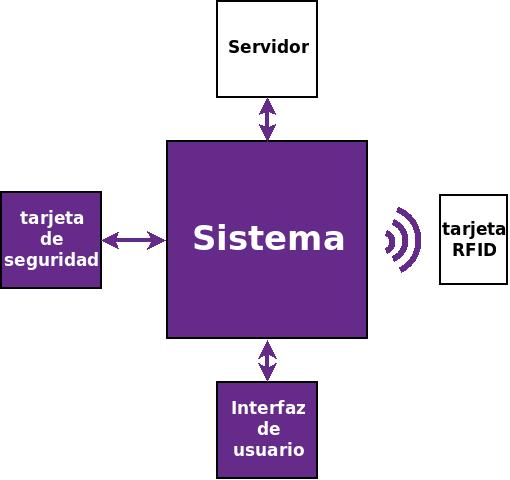
\includegraphics[scale=.3]{../pres_fin/Imagenes/diagrama_def.jpg} 
  	\caption{Bloques que conforman el sistema}\label{sist_gral} 
  \end{center}		 
\end{figure}

De los conceptos antes mencionados, se decidió implementar los bloques correspondientes al 
sistema que incluye el lector/escritor de tarjetas RFID, el lector/escritor de tarjetas 
de seguridad y la interfaz de usuario.
No fueron implementados los bloques relativos al servidor y las tarjetas RFID.


Las partes implementadas forman un prototipo de sistema embebido que interactúa con tarjetas RFID,
permitiendo consultar y/o acreditar saldo en las mismas.
El mecanismo de transferir saldo en las tarjetas RFID mediante éste dispositivo, se encuentra
desacoplado del sistema de pago de dinero, el cual podría efectuarse a través de una red de pagos,
mensajes de texto, web, etc, esto último no forma parte de este proyecto por tanto no fue implementado.



%----------------------------------------------------------------------
% SECTION II: Objetivo
%----------------------------------------------------------------------
\section{Objetivo}
El objetivo del proyecto es la fabricación de un prototipo de sistema embebido capaz de consultar y recargar tarjetas. Para esto, como se mencionó en la introducción, deberá lograr establecer comunicación con tarjetas  como las utilizadas en el Sistema de Transporte Metropolitano (comunicación RFID a 13,56 MHz), con tarjetas de contacto (módulo de seguridad SAM), y con el usuario a través de una interfaz simple.


Esto implica entonces la fabricación de dos lectores/escritores de tarjetas, uno para tarjetas RFID (sin contacto) y
otro para tarjetas con contacto (SAM), una interfaz para el usuario capaz de informar el estado de la transacción
mediante mensajes adecuados, y la utilización de un sistema basado en un microprocesador para controlar los periféricos
y realizar las operaciones. Esto último implica además el desarrollo del software para que todo funcione adecuadamente.



%----------------------------------------------------------------------
% SECTION III: Hardware
%----------------------------------------------------------------------
\section{Hardware}
En una primera instancia se pretendía utilizar únicamente el dispositivo OpenPCD \cite{OpenPCD}, ya que el mismo cuenta con un microcontrolador de la familia ARM, el AT91SAM7S128. Una vez estudiado se llegó a la conclusión que no permitía la instalación de un sistema operativo GNU/Linux, ya que el mismo precisa más de 4 MB de RAM para poder hacer algo útil. Otra desventaja encontrada fue que sólo tiene un puerto I2C como forma de conectar periféricos.

Surgió entonces la necesidad de usar una SBC como dispositivo capaz de ejecutar un sistema operativo y las aplicaciones necesarias para que el dispositivo cumpla con los requerimientos exigidos.

Fue necesario entonces descartar el uso del dispositivo OpenPCD y dar lugar a un diseño propio del lector/escritor de tarjetas RFID, utilizando para esto el integrado CL RC632 de Philips.

Se pensó entonces en diseñar la arquitectura que consta de SBC + lector de tarjetas RFID + lector de tarjeta de contacto + display + buzzer + leds.

En la figura \ref{Fig:HW_GRAL} se muestra un diagrama de bloques correspondiente a la arquitectura seleccionada:

\begin{figure}[h]
\centering
  \begin{center}
  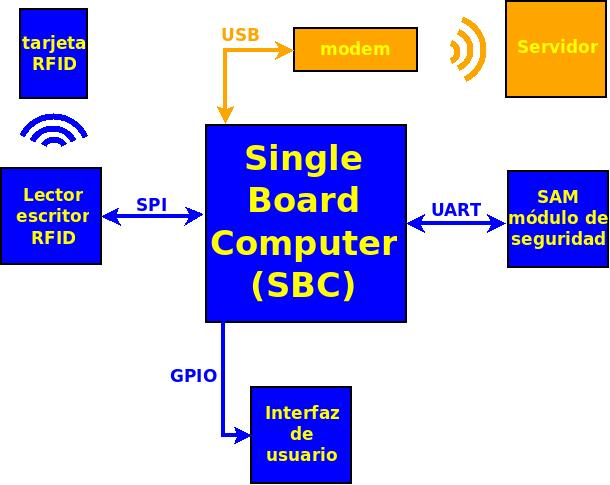
\includegraphics[scale=.3]{../docs/Imagenes/diagrama_rf2.jpg} 
  \end{center}
  \caption{Diagrama de bloques de la arquitectura seleccionada}\label{Fig:HW_GRAL} 
\end{figure}


Los bloques oscuros serán implementados, no así los claros.

La comunicación con un servidor no está implementada por quedar fuera del alcance del proyecto.

\subsection{Elección de hardware}
%\begin{itemize}
%\item SBC
\subsubsection{SBC}
En primera instancia se confeccionó una lista con posibles candidatas de SBC disponibles
en el mercado internacional, teniendo en cuenta factores como: precio, puertos de I/O, memoria RAM, memoria Flash, puertos USB, soporte para GNU/Linux, entre otros.
Se definieron una serie de requisitos mínimos necesarios para seleccionar de la lista la SBC que más se adecuara a la arquitectura definida.
Para la comunicación con el resto de los módulos será necesario: una interfaz UART para el módulo de seguridad (SAM); una interfaz SPI para el módulo lector/escritor RFID (CL RC632 de Philips); 20 GPIO para display, leds, buzzer, otros; 1 USB host previendo una futura conexión de un modem 3G (intercambio de datos con un servidor). En cuanto a la memoria disponible debe ser de 32 MB de RAM y 8 MB de flash para un funcionamiento aceptable. Es conveniente, pensando a futuro, que el procesador trabaje a una frecuencia no menor a 200 MHz.
Dado el presupuesto estimado para el proyecto, el precio no debe superar los 150 dólares en origen.
Como requisito adicional se exigió que existiera un foro actualizado y soporte técnico que permitiera evacuar dudas.

Finalmente, la SBC seleccionada para trabajar fue la Beagleboard rev.C4.

Las características generales de la BeagleBoard son: cuenta con un procesador \\
OMAP3530 de 720 MHz con arquitectura ARM. Posee  memoria NAND-flash de 256 MB y memoria ROM de igual tamaño. Tiene una ranura adicional para extender la memoria a través de una memoria SD. Entre otras cosas cuenta con un puerto USB OTG, un puerto USB host, un bloque de expansión de 28 pines (con señales a 1,8 Volt), puerto JTAG, conector RS232, etc.\\
En lo que respecta a la potencia disipada, la Beagleboard tiene un consumo de pico de 2W, y un consumo promedio de 560mW \cite{consumo1} \cite{consumo2}.

%\item 
\subsubsection{VLT - Conversor de Voltajes}
La placa de circuito impreso VLT consta básicamente de dos conectores, uno de ellos permite la conexión con la Beagleboard y el otro la conexión con el restante hardware el cual se encuentra intergrado en un PCB llamdo SCUI. Ambos conectores no se encuentran directamente interconectados entre sí a través de pistas, pues para el caso particular de Beagleboard fue necesario incorporar conversores de tensión que permitieran el traslado del nivel de tensión desde 1,8 Volt que usa esta SBC, a las tensiones con las que operan los periféricos, ya sea 3,3 o 5 Volt.


%\item 
\subsubsection{Lector de tarjeta de contacto}

Está compuesto por un conversor full duplex a half duplex el cual se encuentra conectado a uno de los puertos UART de la SBC a través del módulo VLT, que se describió en el punto anterior. Este conversor permite la transmisión de datos directamente entre la tarjeta y la SBC, sin necesidad de intercalar un ASIC para el manejo de tarjetas del tipo ISO7816. Cuenta también con un oscilador para alimentar la entrada de reloj de las tarjetas. La entrada de control (OE) del oscilador operada desde la SBC permite poner la salida de reloj en tercer estado, cosa muy útil a la hora de cumplir con la secuencia de inicialización de las tarjetas descritas en el estándar. Se cuenta con un zócalo para insertar la tarjeta de contacto.


%\item 
\subsubsection{Interfaz de usuario}

Está compuesta por tres leds (verde, amarillo y rojo), buzzer y un display LCD16x2 donde son desplegados los mensajes que indican al usuario la operación que se efectúa sobre su tarjeta Mifare.


%\item 
\subsubsection{Lector de tarjetas RFID}

Este módulo es el encargado de la comunicación con las tarjetas RFID que cumplen con la norma ISO14443. Consta básicamente de cuatro secciones entre las que se encuentran: el integrado CL RC632; el filtro EMC, el circuito de adaptación de impedancia (matching); y el inductor de la antena. 
El ASIC CL RC632 permite, por un lado la comunicación digital con un microprocesador a través de su puerto de datos y por el otro lado la transmisión de datos hacia la antena que emitirá la señal RF para la comunicación con las tarjetas ISO14443.

Lo que se llama propiamente antena RF está conformada por el circuito de adaptación de impedancia (matching) y por el inductor ubicado en el circuito impreso, que propaga el campo magnético para lograr el acoplamiento necesario entre lector y tarjeta, de aquí la sigla PCD (Proximity Coupling Device).
%\end{itemize}



%----------------------------------------------------------------------
% SECTION IV: Software
%----------------------------------------------------------------------
\section{Software}

\subsection{Introducción}
Se debe destacar que todo el desarrollo de software se basó exclusivamente en herramientas de software libre. La distribución GNU/Linux elegida para el sistema embebido se llama Angström. Esta distribución es muy usada en aplicaciones que utilizan una Beagleboard como SBC y cuenta con una gran cantidad de bibliotecas implementadas en lenguaje C, que permiten gran escalabilidad a la hora de incorporar nuevos periféricos en la aplicación.


\subsubsection{Sistema Operativo}
En el arranque, la Beagleboard tiene la posibilidad de buscar el bootloader y el kernel en memoria NAND, o en dispositivos extraíbles tales como memorias USB o memorias SD. Para el sistema RF$^{2}$, se eligió un arranque a través de una memoria SD ya que es fácil de manipular.

En la figura \ref{Fig:SD} se puede ver como queda distribuida la memoria SD con las distintas partes
que conforman el sistema operativo. 

\begin{figure}[h]
\centering
  \begin{center}
  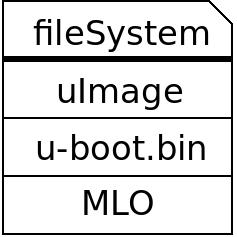
\includegraphics[scale=.4]{../docs/Imagenes/sd.jpg} 
  \end{center}
  \caption{Memoria SD para funcionar en Beagleboard}\label{Fig:SD} 
\end{figure}

En la memoria SD se pueden distinguir dos particiones, una en formato FAT32 y otra
en formato ext3. La partición en FAT32 es llamada “de arranque”, y es donde se encuentra 
el bootloader (MLO, u-boot.bin) y la imagen comprimida del kernel (uImage). 
La partición en ext3 es donde se encuentra el sistema de archivos (fileSystem) asociado con la distribución elegida.


\subsection{Herramientas utilizadas en el desarrollo del sistema}

\subsubsection{Introducción}
Para la elección de las herramientas se tomó como primer criterio de decisión el hecho que sean libres, así como las experiencias de otras personas que ya han transitado caminos comunes, consultando y participando en foros activos.


A continuación se detallan algunas de las herramientas utilizadas para el desarrollo del sistema. 

\subsubsection{MLO, u-boot.bin y uImage}
No fue necesario generar el MLO debido a su simpleza, puesto que el binario precompilado realiza bien su función.

El u-boot.bin y el uImage fueron generados con la herramienta de desarrollo y compilación OpenEmbedded-Bitbake que es una fusión de dos herramientas: OpenEmbedded, herramienta para construcción y mantenimiento de distribuciones, y Bitbake, herramienta de compilación similar al Make que automatiza la construcción de ejecutables entre otros. Esto es, OpenEmbedded utiliza Bitbake para su objetivo. OpenEmbedded-Bitbake es una herramienta muy potente y difícil de aprender al principio. Luego de entendido su principio de funcionamiento se hace muy simple su uso.


\subsubsection{FileSystem}
Para la generación del fileSystem de Angström, se utilizó la herramienta web Narcissus disponible en la página de Angström.


\subsubsection{Crosscompilación}
Para la crosscompilación se utilizó el SDK generado por Narcissus y la herramienta Make para generar los archivos necesarios.

\subsubsection{Depuración de código}
Para la depuración, se utilizó la herramienta GDB del proyecto GNU. 


\subsubsection{Bibliotecas}

\begin{itemize}
\item pcsc-scan 
Esta aplicación fue utilizada para testear el lector de tarjetas de contacto.
\item  librfid-tool 
Esta herramienta fue utilizada para testear lectores/escritores de tarjetas RFID.
\end{itemize}


\subsection{Desarrollo}

\subsubsection{MLO}
Como se mencionó anteriormente, no fue necesario generar el MLO debido a que la Beagleboard viene con uno pre-instalado, y en caso que no funcione en forma correcta se puede descargar desde un repositorio de Angström. 

\subsubsection{Multiplexado de pines}
El microprocesador OMAP3530 tiene muchos pines con distintas interfaces entre las
que se cuentan puertos UART, SPI, GPIO, etc., pero no todos son accecibles desde la Beagleboard. 
Para poder acceder a algunos de estos puertos del microprocesador, existe en la placa de la
Beagleboard un bloque de expansión de 28 pines.


Por defecto, en el bloque de expansión no se encuentran las señales que se quieren. Esto 
lleva a que se tenga que modificar el estado inicial de los pines. 
Existen dos formas de modificar los pines de modo de tener las señales que se precisan. Una de ellas es modificar el bootloader y la otra es modificar el kernel. Esto implica cambios en los archivos fuentes y posterior compilación que genere los nuevos binarios u-boot o uImage. 


Para la modificación de las señales disponibles en el bloque de expansión se decidió modificar el u-boot, ya que la modificación por u-boot es más intuitiva y por experiencia se sabe que lo que más se actualiza y/o modifica es el kernel. 

\subsubsection{u-boot}
Como se mencionó anteriormente, en el u-boot se realizó la configuración de los pines del bloque de expansión de la Beagleboard. 
Cada pin del bloque de expansión tiene varias funcionalidades asociadas, y la configuración de la 
funcionalidad depende de un multiplexado modificable a nivel de software. Esto es, dependiendo del “modo de pin” elegido, la función que se obtiene en dicho pin.

Pese a que en la literatura y foros, se plantea lo contrario, no fue posible establecer los atributos “valor” y “dirección” de los pines GPIO mediante la modificación planteada. Lo que sí cambia efectivamente es el modo del pin, permitiendo obtener las interfaces adecuadas en el bloque de expansión.

\subsubsection{uImage}
La versión del kernel elegida fue la 2.6.32 ya que en el momento que se comenzó el desarrollo era la versión más estable.
En algunos casos, no aparecen algunas de las interfaces configuradas, lo que lleva a modificar los fuentes del kernel para que esto así suceda. Este fue el caso de la interfaz SPI que no quedó mapeada en /dev pese a que había sido configurada en los fuentes del u-boot. También hubo problemas con los atributos “valor” y “dirección” de los GPIO, como se mencionó anteriormente. Adicionalmente hacía falta un módulo para simular una conexión ethernet sobre una interfaz USB para establecer una conexión entre la Beagleboard y un PC, que emula una tarjeta de red por software.
Todo esto llevó a que se tuvieran que modificar los archivos fuente del kernel.

\subsubsection{FileSystem}

Como se mencionó anteriormente, el fileSystem se generó a partir de la herramienta web Narcissus.\\
En el fileSystem es donde se encuentran los paquetes y programas ya instalados. Cuanto más programas se instalen más grande será en tamaño el fileSystem.

\subsubsection{Bibliotecas}

\leftline{\bf{Software para el manejo de GPIO}}

Este módulo de software fue realizado desde cero, basándose en el fileSystem virtual SYSFS para el control de GPIOs \cite{gpio} \cite{gpioK}, esto permite que el código pueda ser portado a cualquier otro sistema que use GNU/Linux y que disponga de este tipo de hardware.

\bigskip
\leftline{\bf{Software para comunicación SAM}}

Como fue descrito en la sección de hardware, el lector de tarjetas de contacto tiene una interfaz serial pura para la transferencia de datos con las tarjetas. En base al diseño hardware elegido, las capas de software sobre las que se decidió trabajar son las que se detallan en la figura \ref{Fig:capas}. 

\begin{figure}[h]
\centering
  \begin{center}
  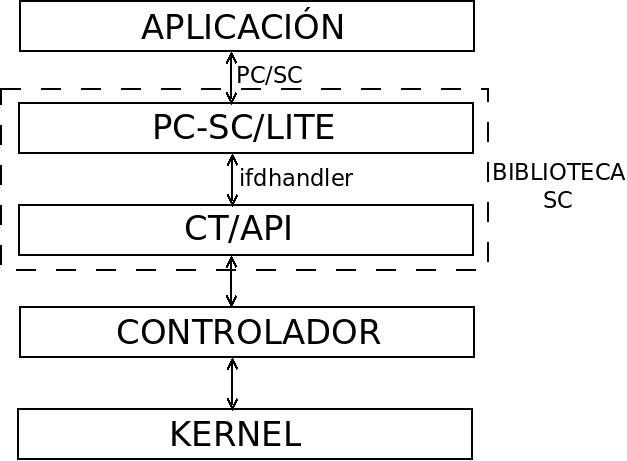
\includegraphics[scale=.35]{../docs/Imagenes/SW_sc1.jpg} 
  \end{center}
  \caption{Capas de software de trabajo}\label{Fig:capas} 
\end{figure}


A continuación se describen las capas asociadas a la figura \ref{Fig:capas}.


\leftline{Controlador:}
El kernel es el encargado de manipular directamente los registros del puerto serial, las interrupciones que desde éste se generan y la ISR para atender las interrupciones.
La implementación del controlador del lector de tarjetas se basó en el controlador serial de GNU/Linux a través de su estructura “termios” \cite{termios}. Esta estructura permite configurar todos los parámetros necesarios para la comunicación serial como ser, baud rate, cantidad de bits por byte, bit de paridad, bit de parada entre otros. Las funciones read y write permiten la lectura y escritura de los bytes de datos que son recibidos y transmitidos por el puerto serial.


CT/API (Card Terminal / Application Programming Interface):
Por encima del controlador serial se encuentra CT/API \cite{ctapi}, una interfaz definida por varias empresas (entre las que se incluye Telekom Alemania) en la década de los noventa, que permite encapsular el controlador específico de cada lector de tarjetas, de manera que la aplicación final no se vea afectada al cambiar un lector por otro.
Esta interfaz de programación está formada tan solo por tres funciones, CT\_init, CT\_data y CT\_close, que permiten la inicialización del lector, la transferencia de datos entre \\
host/lector o host/tarjeta (host se refiere a la SBC o PC donde se encuentra conectado el lector de tarjetas de contacto) directamente y el cierre de la comunicación.\\


\leftline{IFDHandler:}
El siguiente componente en este stack de capas es ifdhandler; no es otra cosa que un conjunto de funciones formando una API, empleada por pcsclite para encapsular el manejo del hardware de lectores cuyos fabricantes quieran cumplir con las especificaciones PC/SC. Una ventaja importante de esta API es que le permite a pcsclite operar tanto con lectores de puerto serial como con lectores de puerto USB.
Esta capa de software podría usarse directamente sobre el controlador del lector, prescindiendo de CT/API, aunque se decidió mantenerla por motivos de simplicidad ya que sólo es necesario sustituir la capa de aplicación por las restantes capas superiores como se indica en la figura \ref{Fig:capas}.


Las funciones que contiene esta capa de software fueron modificadas para que contengan a su vez las funciones de CT/API, y de esta manera hacer más fácil de integrar el controlador del lector con la biblioteca PCSCLite.


\leftline{PCSCLite:}
Por arriba de ifdhandler se encuentra la biblioteca pcsclite, ésta contiente todas las funciones necesarias para establecer la comunicación con un lector y la tarjeta conectada a éste último.


\leftline{Aplicación final:}
Por arriba de todas las capas descritas antes, se encuentra la aplicación del prototipo que hace uso de las funciones suministradas por pcsclite y donde se encuentran definidos los comandos APDU específicos con los que opera la tarjeta de contacto.

\bigskip
\leftline{\bf{Software RFID}}
librfid es una biblioteca de software libre para manejo de lectores/escritores RFID. Implementa el stack de protocolos del lado del dispositivo lector/escritor ISO 14443A, ISO 14443B, ISO 15693, Mifare Ultralight y Mifare Classic.

Entre los lectores soportados están, OpenPCD y algunos modelos Omnikey, éstos con interfaz de conexión USB. Además tiene soporte para cualquier otro lector con comunicación directa con el CL RC632 mediante la interfaz SPI y es por esta razón que se tuvo en cuenta.

El manejo de librfid es de bajo nivel y se comunica directamente con el kernel utilizando el módulo spidev. Librfid-tool implementa funciones de más alto nivel que hacen uso de las funciones de bajo nivel de la librfid. La estrucrura de software comentada se muestra en la figura \ref{sw_RFID}.

\begin{figure}[h]
\centering
  \begin{center}
  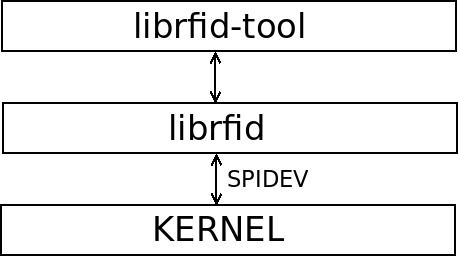
\includegraphics[scale=.4]{../docs/Imagenes/librfid-tool.jpg} 
  \end{center}
  \caption{Capa de software RFID}\label{sw_RFID} 
\end{figure}


Después de estudiadas las funciones que provee la herramienta librfid-tool, se estudió la posibilidad de su uso para la aplicación RF$^{2}$. 

Aunque sus funciones  son muy útiles, la gran mayoría no sirven completamente para la aplicación RF$^{2}$ debido a que fueron definidas para otros propósitos. 

Es de interés, que la herramienta librfid-tool siga manteniendo sus funcionalidades y pueda convivir con la aplicación RF$^{2}$, por lo que no se modificó el contenido de ninguna función de la herramienta. En el caso que alguna función fuera mayormente utilizable, se procedió a crear una nueva con los cambios necesarios.

Se implementaron la mayoría de las funciones, logrando compatibilidad con la biblioteca librfid. Entre las funciones creadas están las asociadas con la tarjeta RFID: autenticación según el tipo de clave, búsqueda de tarjetas próximas al lector, lectura y escritura de bloques de memoria, obtención del UID, etc.

\subsubsection{Aplicación final}

Para el desarrollo de la aplicación RF$^{2}$ se decidió trabajar sobre los fuentes de la herramienta librfid-tool, ya que maneja varias funciones de utilidad y es de ayuda a la hora de compilar para el armado de una aplicación completa. Se mantuvieron todas las opciones de la herramienta ya que son útiles, y pueden ayudar en un futuro para establecer orígenes de fallas. No se modificó ninguna función de la aplicación original y cuando fue necesaria alguna modificación, se procedió a implementar una nueva.

En la figura \ref{Fig:SW} se detallan las capas de software del sistema RF$^{2}$.

\begin{figure}[h]
\centering
  \begin{center}
  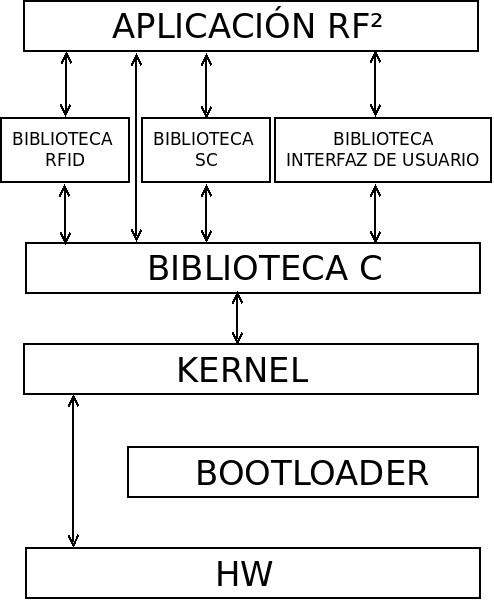
\includegraphics[scale=.35]{../docs/Imagenes/SW.jpg} 
  \end{center}
  \caption{Capas de software del sistema RF${^{2}}$}\label{Fig:SW} 
\end{figure}

\newpage
\leftline{\bf{Modificaciones en librfid-tool}}

Se implementó una función de inicialización, la cual inicializa todos los periféricos al arrancar la aplicación RF$^{2}$.

En librfid-tool.h se definieron constantes simbólicas para hacer configurable al sistema. 

Se agregó una nueva opción (n) en el main de la aplicación librfid-tool que llama a la función principal(). Ésta, es la función principal de la aplicación RF$^{2}$, la cual se ejecuta en loop.
% y se basa en el diagrama de flujo de la figura \ref{Fig:HW}. 
De este modo no se modifica el main original de librfid-tool (sólo se agrega la opción n) y se dejan las opciones por defecto.

\bigskip
\leftline{\bf{Funcionamiento general de la aplicación}}

Se desarrolló una estructura de directorios de forma que el sistema sea modular, esto es, cualquier cambio requerido en algún módulo del sistema, no afecta al resto.

De las funciones, salvo dos, todas fueron realizadas por el grupo de trabajo.


%----------------------------------------------------------------------
% SECTION V: Costos
%----------------------------------------------------------------------
\section{Costos}

El costo total del proyecto asciende aproximadamente a 1385 dólares, habiendo 
estimado un gasto total de 1500 dólares.

En cuanto al costo de fabricación de los PCB, se puede decir
que las diferencias en precio son sustanciales, dependiendo
del origen del fabricante. 

El costo por unidad con los PCB hechos en Uruguay es de aproximadamente U\$S375, si los PCB se fabricaran en China el costo sería de unos U\$S242.



%----------------------------------------------------------------------
% SECTION VI: Conclusiones
%----------------------------------------------------------------------
\section{Conclusiones}
El mundo de la tecnología RFID está poco explorado en nuestro país, éste 
tal vez sea el primer proyecto que incluye el diseño y fabricación de un 
lector/escritor RFID capaz de operar con tarjetas sin contacto en la banda de
frecuencia de 13,56 MHz.

El aporte realizado en este campo es tan solo una primera aproximación y aún 
queda mucho por hacer al respecto. Sobre este proyecto en particular es
necesario mejorar varios aspectos antes de pasar de la fase de prototipo
a la de producción.


Repasando en particular los criterios de éxito, el proyecto ha resultado satisfactorio
porque se logró construir un dispositivo capaz de consultar y recargar tarjetas RFID,
aunque la solución alcanzada no sea estrictamente igual a la propuesta en el comienzo.



% do the biliography:
\bibliographystyle{IEEEbib}
%\bibliographystyle{plain}
%\include{biblio}
\begin{thebibliography}{10}

\bibitem{OpenPCD} OpenPCD, http://www.openpcd.org/, agosto 2011.

\bibitem{consumo1} Consumo de Beagleboard, http://elinux.org/BeagleBoardFAQ\\
\#Power\_usage, agosto 2011.

\bibitem{consumo2} Consumo de Beagleboard, http://www.h-online.com/news-\\
/forum/S-Power-consumption-under-2W/forum-110345/msg-14369911/read/, agosto 2011.

\bibitem{gpio} GPIO, http://www.avrfreaks.net/wiki/index.php/Documenta\\
tion:Linux/GPIO\#Interfaces\_explained, agosto 2011.

\bibitem{gpioK} Kernel GPIO, http://kernel.org/doc/Documentation/gpio.txt, agosto 2011.

\bibitem{termios} termios, http://pubs.opengroup.org/onlinepubs/007908799/xsh\\
/termios.h.html, agosto 2011.

\bibitem{ctapi} Application Independent CardTerminal Application Programming Interface for ICC Applications; 
Deutsche Telekom AG / PZ Telesec, GMD - Forschungszentrum Informationstechnik GmbH, TÜV Informationstechnik GmbH, TELETRUST Deutschland e.V., 30.10.1996.

\end{thebibliography}

% where ``my-bibliography-file.bib'' is the name of the file with all the 
% BibTeX entries.

% do the biographies...
%\begin{biography}{Autor}
%Aquí se detalla la biografía del autor.
%\end{biography}

% If you want a picture with your biography, then specify the name of
% the postscript file in square brackets. That is, uncomment the
% following three lines and change the name of "face.ps" to the name of 
% your file.
%\begin{biography}[face.ps]{Gregory L. Plett}
%  A bio with a face...
%\end{biography}

%----------------------------------------------------------------------
% FIGURES
%----------------------------------------------------------------------
% There are many ways to include figures in the text. We will assume
% that the figure is some sort of EPS file.
%
% The outdated packages epsfig and psfig allow you to insert figures
% like: \psfig{filename.eps} These should really be done now using the
% \includegraphics{filename.eps} command.  
%
% i.e.,
%
% \includegraphics{file.eps}
%
% whenever you want to include the EPS file 'file.eps'. There are many
% options for the includegraphics command, and are outlined in the
% on-line documentation for the "graphics bundle". Using the options,
% you can specify the height, total height (height+depth), width, scale,
% angle, origin, bounding box "bb",view port, and can trim from around
% the sides of the figure. You can also force LaTeX to clip the EPS file
% to the bounding box in the file. I find that I often use the scale,
% trim and clip commands.
% 
% \includegraphics[scale=0.6,trim=0 0 0 0,clip=]{file.eps}
% 
% which magnifies the graphics by 0.6 (If I create a graphics for an
% overhead projector transparency, I find that a magnification of 0.6
% makes it look much better in a paper), trims 0 points off
% of the left, bottom, right and top, and clips the graphics. If the
% trim numbers are negative, space is added around the figure. This can
% be useful to help center the graphics, if the EPS file bounding box is
% not quite right.
% 
% To center the graphics,
% 
% \begin{center}
% \includegraphics...
% \end{center}
% 
% I have not yet written good documentation for this, but another 
% package which helps in figure management is the package ieeefig.sty,
% available at: http://www-isl.stanford.edu/people/glp/ieee.shtml
% Specify:
% 
%\usepackage{ieeefig} 
% 
% in the preamble, and whenever you want a figure,
% 
%\figdef{filename}
% 
% where, filename.tex is a LaTeX file which defines what the figure is.
% It may be as simple as
% 
% \inserteps{filename.eps}
%
% or
% \inserteps[includegraphics options]{filename.eps}
% 
% or may be a very complicated LaTeX file. 

\end{document}
